\section{Uncertainty Analysis, Counting Statistics, and Detection}
\subsection{Uncertainty Analysis}
\subsubsection{Characterization of Data}
With $N$ independent measurements of the same physical quantity:
\begin{itemize}
    \item Experimental mean: $\overline{x_e}=\frac{1}{N}\sum_{i=1}^Nx_i$
    \item Residual: $d_i=x_i-\overline{x_e},\text{ with }\sum_{i=1}^Nd_i=0$
    \item Deviation: $\epsilon_i=x_i-\overline{x}$, note that $\overline{x}$ is the true mean 
    \item Sample variance: $s^2=\overline{\epsilon^2}=\frac{1}{N}\sum_{i=1}^N(x_i-\overline{x})^2=\frac{1}{N-1}\sum_{i=1}^N(x_i-\overline{x_e})^2$
    \item Standard Deviation: $\sigma^2=\frac{1}{N}\sum_{i=1}^N(x_i-\overline{x})^2=\frac{1}{N-1}\sum_{i=1}^N(x_i-\overline{x_e})^2$, or $\sigma^2\approx\overline{x_i^2}-(\overline{x_e})^2$\\
    The standard deviation is also known as the external uncertainty in the mean.
\end{itemize}
\subsubsection{Internal and External Uncertainties}
\begin{itemize}
    \item The uncertainty in the mean (internal uncertainty) is $\sigma_{\text{internal}}=\sigma/\sqrt{N}$
    \item Assuming different uncertainties $\sigma_i$ for $x_i$:
    \begin{itemize}
        \item The weighted mean $\overline{x_w}=\left(\sum_{i=1}^Nx_i\right)/\left(\sigma_i^2\sum_{i=1}^N1/\sigma_i^2\right)$
        \item The error in the weighted mean $\sigma_{\text{internal}}=1/\sqrt{\sum_{i=1}^N1/\sigma_i^2}$\\, or $\left(1/\sigma_\text{internal}^2\right)=\sum_{i=1}^N\left(1/\sigma_{x_i}^2\right)$
        \item The external uncertainty $\sigma_\text{external}=\sigma_\text{internal}\sqrt{\frac{\sum(x_i-\overline{x})^2/\sigma_i^2}{N-1}}$
    \end{itemize}
    
\end{itemize}
\subsubsection{Error Propagation Rules}
\begin{itemize}
    \item Assume $N$ independent measurements of the same physical quantity, to which $F$ is related by $F=F(x_1,x_2,...)$:\\
    then the uncertainty in F is given by $\sigma_F^2=\sum_{i=1}^N\left(\frac{\partial F}{\partial x_i}\right)^2\sigma^2_{x_i}$
    \item Examples
    \begin{itemize}
        \item Sum and differences: $\sigma_{x+y}=\sigma_{x-y}=\sqrt{\sigma_x^2+\sigma_y^2}$
        \item Multiplication and division by constant: $\sigma_{Kx}=K\sigma_x$
        \item Multiplication: $\sigma_{x\cdot y}=(x\cdot y)\sqrt{\left(\sigma_x/x\right)^2+\left(\sigma_y/y\right)^2}$
        \item Division: $\sigma_{x/y}=({x}/{y})\sqrt{\left(\sigma_x/x\right)^2+\left(\sigma_y/y\right)^2}$
    \end{itemize}
    \item Counting Rate ($R$)
    \begin{itemize}
        \item[] $R=n/T$ and $\sigma_n=\sqrt{n}\;\Rightarrow\;\sigma_R=\sqrt{n}/{T}=\sqrt{R/T}$
        \item[] $R_S=R_{S+B}-R_B\;\Rightarrow\;\sigma_{R_S}=\sqrt{\frac{n_{S+B}}{T_{S+B}^2}+\frac{n_{B}}{T_{B}^2}}=\sqrt{\frac{R_{S+B}}{T_{S+B}}+\frac{R_B}{T_B}}$
    \end{itemize}
\end{itemize}
\subsubsection{Rounding of Values}
Rounding to 1-2 significant figures in the uncertainty, demonstrated by the following examples:
\begin{center}
\begin{tabular}{c c c}
    Raw value & $n=1$ & $n=2$\\
    \hline
    $5.73297251\pm0.01477602$ &  $5.73\pm0.01$ & $5.733\pm0.015$ \\
    $314775089\pm4500284$ & $(3.15\pm0.05)\times10^8$ & $(3.148\pm0.045)\times10^8$ \\
    $255\pm73$ & $(2.6\pm0.7)\times10^2$ & $255\pm73$
\end{tabular}  
\end{center}
\subsection{Counting Statistics}
\subsubsection{Statistical Models}
\begin{itemize}
    \item Binomial distribution
    \begin{itemize}
        \item The most general of all listed here. Given probability $p$ of an event in a single trial, the probability of $x$ events in $n$ trials is given by\\
        $P(x)=\frac{n!}{x!(n-x)!}p^x(1-p)^{n-x}$
        \item[] $\overline{x}=np$
        \item[] $\sigma^2=np(1-p)=\overline{x}(1-p)$
        \item[] $\sum_{x=0}^nP(x)=1$
        \item Though computationally intensive, radioactive decay can be described with a very large $n$ and $p=1-\exp(-\lambda t)$
    \end{itemize}
    \item Poisson distribution
    \begin{itemize}
        \item If $p$ of the binomial distribution is small and constant ($p\ll1$), it can be reduced to the Poisson distribution. For example, when a count interval is short compared with the half-life of the source.
        \item[] $P(x)=\frac{(\overline{x})^xe^{-\overline{x}}}{x!}$
        \item[] $\overline{x}=np$
        \item[] $\sigma^2=np=\overline{x}$
        \item[] $\sum_{x=0}^nP(x)=1$
        \item Note that to characterize a Poisson distribution, only one parameter is needed, that is the product of $n$ and $p$. With only the mean value of the distribution ($\overline{x}$), the entire distribution can be constructed.
    \end{itemize}
    \item Normal distribution
    \begin{itemize}
        \item If in addition to $p\ll1$, the mean value of the distribution is large enough ($np\gg1$), the distribution can be further simplified to a normal (Gaussian) distribution.
        \item[] $P(x)=\frac{1}{\sqrt{2\pi\overline{x}}}\exp\left(-\frac{(x-\overline{x})^2}{2\overline{x}}\right)=\frac{1}{\sigma\sqrt{2\pi}}\exp\left(-\frac{(x-\overline{x})^2}{2\sigma^2}\right)$
        \item[] $\overline{x}=np$
        \item[] $\sigma^2=np=\overline{x}$
        \item[] $\sum P(x)=1$
    \end{itemize}
\end{itemize}
\subsubsection{Confidence}
\begin{itemize}
    \item Estimation of the precision of a single measurement:
    \begin{itemize}
        \item When only one measurement with result $x$ is made, but we would like to associate some uncertainty with the measurement, we have $\overline{x}=x$ and $\sigma=\sqrt{x}$
        \item The ranges of values $x\pm\sigma=x\pm\sqrt{x}$, $x\pm2\sigma$, and $x\pm3\sigma$ will contain the true mean ($\overline{x}$ of the predicted probability distribution function $P(x)$) with 68.3\%, 95.5\%, and 99.7\% probability respectively, according to the normal distribution function. 
    \end{itemize}
    \item Confidence limits
    \begin{itemize}
        \item A confidence limit expresses the probability that a measurement will be within a certain range around a chosen value. Assuming a normal distribution, the confidence interval around the mean\\
        $P(x<x_a)=\int_{\overline{x}-x_a}^{\overline{x}+x_a}\frac{1}{\sigma\sqrt{2\pi}}\exp\left(-\frac{(x-\overline{x})^2}{2\sigma^2}\right)$
        \item This range $x_a$ is often expressed in terms of $k$ standard deviations from the mean, as $x_a=\overline{x}\pm k\sigma$
        \item As discussed above, $k=1$ means that 68.3\% of measurements will be found to be inside this range. (Similarly, it is 95.5\% for $k=2$, and 99.7\% for $k=3$.)
    \end{itemize}
\end{itemize}
\subsubsection{The \texorpdfstring{$\chi^2$}{Chi-squared} Test}
\begin{itemize}
    \item The Pearson's $\chi^2$ Test provides a quantitative way of matching the distribution of experimental data to an appropriate statistical model. Usually, we'll match to a Poisson or normal distribution, $P(x)$ with $\overline{x}=\overline{x_e}$
    \item We would also like to compare the value of the sample variance  $s^2$ and the predicted variance of $P(x)$, which is $\sigma^2=\overline{x}$
    \item With $N$ measurements, $\chi^2=\frac{1}{\overline{x_e}}\sum_{i=1}^{N}(x_i-\overline{x_e})^2=\frac{1}{\overline{x}}\sum_{i=1}^{N}(x_i-\overline{x})^2$
    \item By comparing to the expression of the sample variance $s^2$ given in section 5.1.1, we can see that $\chi^2=\frac{(N-1)s^2}{\overline{x}}$\\
    If the fluctuation in the experimental data is closely modeled by the Poisson distribution, then $s^2\approx\sigma^2=\overline{x}$\\
    Therefore, the degree to which the expression $(s^2/\overline{x})$ deviates from unity, or the degree to which $\chi^2$ differs from $(N-1)$ is a measure of the departure of the data from the predicted Poisson distribution.
    \item The statistical of degree freedom $\nu$ of the system is $(N-1)$ (since $\overline{x}$ is calculated from the same set of data). With the values of $\nu$ and $\chi^2$, we can read off the $p$ from a $\chi^2$ distribution table.
    \item $p$ is defined as the probability that a random sample from a true Poisson distribution would have a larger value of $\chi^2$ than the value calculated from the experimental data. A perfect fit to the Poisson distribution would yield $p=0.5$ ; a high $p$ indicates abnormally small fluctuations, and a low $p$ indicates abnormally large fluctuations.
\end{itemize}
\subsubsection{Examples}
\begin{enumerate}
    \item A series of measurements
    \begin{itemize}
        \item Given a series of length measurements:\\
        17.62, 17.62, 17.615, 17.62, 17.61, 17.61, 17.62, 17.625,\\ 17.62, 17.62,
        17.61, 17.615, 17.61, 17.605, 17.61
        \item Assume the data is Gaussian distributed:
        \begin{itemize}
            \item[] Mean: $\overline{x}=17.61533$
            \item[] Standard deviation: $\sigma=5.855\times10^{-3}$
            \item[] Error in the mean: $\sigma(\overline{x})=\sigma/\sqrt{n}=1.5\times10^{-3}$
            \item[] Therefore, the best value: $x=17.616\pm0.002$
        \end{itemize}
    \end{itemize}
    \item Count rates
    \begin{itemize}
        \item Five count rate [counts/min] measurements were made, with counting interval of 1 minute:\\
        2201, 2145, 2222, 2160, 2300
        \item Decay is described by the Poisson distribution:
        \begin{itemize}
            \item[] $\overline{x}=2205.06$
            \item[] $\sigma(\overline{x})=\sigma/\sqrt{n}=\sqrt{\overline{x}/n}=\sqrt{2205.6/5}=21$
            \item[] The count rate is therefore $2206\pm21$ counts/min
        \end{itemize}
        \item The identical result is can be found if one measurement of 5 minutes was performed. (See below)
    \end{itemize}
    \item Consecutive counting
    \begin{itemize}
        \item Assume $N$ repeated counts of the same source with equal counting times. The results are $x_1,\;x_2,\;...,\;x_N$, and their sum $\Sigma=x_1+x_2+...+x_N$
        \item By error propagation, we know $\sigma_\Sigma^2=\sigma_{x_1}^2+\sigma_{x_2}^2+...+\sigma_{x_N}^2$\\
        But we also know $\sigma_{x_i}=\sqrt{x_i}$\\
        $\Rightarrow\;\sigma_\Sigma^2=x_1+x_2+...+x_N=\Sigma$ , and $\sigma_\Sigma=\sqrt{\Sigma}$\\
        This shows that the standard deviation expected for the sum of all the counts is the same as if the measurement had been carried out by performing a single count, with counting interval as the combination of all independent counting times.
        \item The mean of these $N$ measurements is $\overline{x}=\Sigma/N$\\
        By error propagation (division by constant), we can see that \\$\sigma(\overline{x})=\sigma_\Sigma/N=\sqrt{\Sigma}/N=\sqrt{N\overline{x}}/N=\sqrt{\overline{x}/N}$
    \end{itemize}
    \item The null Experiment
    
\end{enumerate}
\subsection{Detection}
\subsubsection{Dead Time}
\begin{enumerate}
    \item Overview
    \begin{itemize}
        \item Finite time to process signals, due to detectors and electronics, causes dead time. Since decay is random, there is always a chance for ``pile-up''.
        \item Figure~\ref{fig:dead_time_models} shows the two commonly used models.
    \end{itemize}
    \begin{figure}[ht]
        \centering
        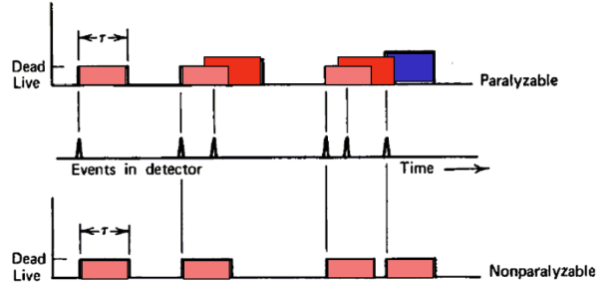
\includegraphics[width=0.6\textwidth]{images/deadtimemodels.png}
        \caption{Visualization of the paralyzable and nonparalyzable models. }
        \label{fig:dead_time_models}
    \end{figure}
    \item Distribution of time intervals between 
    successive events
    \begin{itemize}
        \item Assuming that an event happened at $t=0$, what is the differential probability that the next event will take place within a differential time $dt$ after a time interval of length $t$?
        \begin{itemize}
            \item[] $(I(t)\;dt)$ is the overall probability of the next event taking place in $dt$ after delay of $t$
            \item[] $(P(0))$ is the probability that no events occurred during time from $0$ to $t$
            \item[] $(r\;dt)$ is the probability of an event occurring during $dt$
            \item[] $\Rightarrow\;I(t)\;dt=P(0)\times r\;dt$
        \end{itemize}
        \item Following the form of the Poisson distribution given in section 5.2.1, and since the average number of recorded events during $t$ should be $rt$, 
        \begin{itemize}
            \item[] $P(0)=\frac{(rt)^0e^{-rt}}{0!}=e^{-rt}$
        \end{itemize}
        \item Therefore, $I(t)\;dt=re^{-rt}\;dt$
    \end{itemize}
    \item Paralyzable model
    \begin{itemize}
        \item As shown in figure~\ref{fig:dead_time_models}, in the paralyzable model, all signals will be detected if the time interval between true events exceed the system dead time.
        \item Let $\tau$ be the system dead time,\\
        $m$ be the recorded count rate, and\\
        $n$ be the true interaction rate.
        \item Using the equation from part 2, the probability of intervals larger than $\tau$ can be written as\\
        $P(\tau)=\int_\tau^\infty ne^{-nt}dt=e^{-n\tau}$
        \item Since the observed rate will be equal to the true rate if $t>\tau$, \\
        $m=ne^{-n\tau}$
    \end{itemize}
    \item Non-paralyzable model 
    \begin{itemize}
        \item In the non-paralyzable model, the fraction of all time that the detector is dead is given by $(m\tau)$
        \item The rate at which true events are lost is therefore $(nm\tau)$
        \item Since the rate of losses can also be given as $(n-m)$, we arrive at the expression\\
        $n-m=nm\tau$
        \item The above equation gives $n=m/(1-m\tau)$ and $m=n/(1+n\tau)$
    \end{itemize}
    \item Comparison of dead time models
    \begin{figure}[ht]
        \centering
        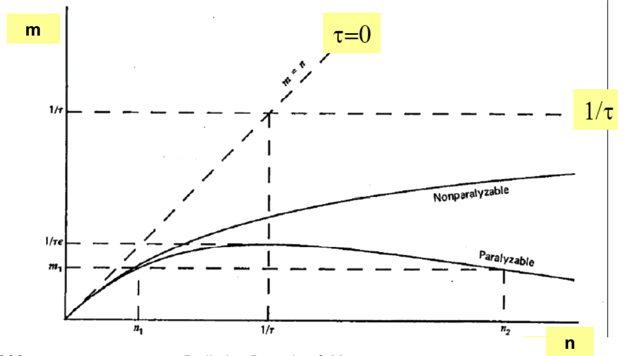
\includegraphics[width=0.6\textwidth]{images/deadtimemodel_comparison.png}
        \caption{Comparison of dead time models. $m$ is observed count rate, $n$ is true count rate.}
        \label{fig:dead_time_models_comparison}
    \end{figure}
    \begin{itemize}
        \item As shown in figure~\ref{fig:dead_time_models_comparison}, at low true count rates, both models given virtually the same observed rate. Mathematically, for $n\ll1/\tau$, 
        \begin{itemize}
            \item Paralyzable: $m=\frac{n}{1+n\tau}\rightarrow n(1-n\tau)$
            \item Non-paralyzable: $m=ne^{-n\tau}\rightarrow n(1-n\tau)$
        \end{itemize}
        \item At high true count rates, the observed count rates can be very different. The non-paralyzable model approaches the asymptotic behavior of $m\rightarrow(1/\tau)$
        \item Beware that in the paralyzable model, the same $m$ can actually correspond to two different $n$ values, since there is a maximum in the curve. (In figure~\ref{fig:dead_time_models_comparison}, $m_1$ can correspond to either $n_1$ or $n_2$) By varying the true rate and observing whether $m$ increases or decreases, the ambiguity can be resolved.
    \end{itemize}
    \item Dead Time Measurements
    \begin{itemize}
        \item Two-source method
        \begin{itemize}
            \item Let $n_1$ and $m_1$ correspond to source 1, $n_2$ and $m_2$ correspond to source 2, and $n_{12}$ and $m_{12}$ correspond to both sources (simultaneously counted). $n_b$ and $m_b$ correspond to background.
            \item True count rates $n_{12}-n_b=(n_1-n_b)+(n_2-n_b)\;\Rightarrow\;n_{12}+n_b=n_1+n_2$\\
            \item Assuming non-paralyzable dead time, $\frac{m_{12}}{1-m_{12}}+\frac{m_b}{1-m_b}=\frac{m_1}{1-m_1}+\frac{m_2}{1-m_2}$\\
            \item If $m_b=n_b=0$, then $\tau=\frac{m_1m_2-\sqrt{m_1m_2(m_{12}-m_1)(m_{12}-m_2)}}{m_1m_2m_{12}}$
            \item With this method, no information regarding source activity or detector efficiency is needed 
        \end{itemize}
        \item Decaying source method
        \begin{itemize}
            \item Paralyzable model:
            \begin{itemize}
                \item[] $n=n_0e^{-\lambda t}$
                \item[] $n=m/(1-m\tau)$
                \item[] $\Rightarrow\;me^{\lambda t}=n_0-n_0m\tau$
            \end{itemize}
            \item Non-paralyzable model:
            \begin{itemize}
                \item[] $m=ne^{-n\tau}$
                \item[] $\ln(m)=\ln(n)-n\tau$
                \item[] $\ln(m)=\ln(n_0e^{-\lambda t})-n_0e^{-\lambda t}\tau=\ln(n_0)-\lambda t-n_0e^{-\lambda t}\tau$
                \item[] $\ln(m)+\lambda t=\ln(n_0)-n_0 e^{-\lambda t}\tau$
            \end{itemize}
        \end{itemize}
    \end{itemize}
\end{enumerate}
\subsubsection{Decision Making}
\begin{enumerate}
    \item The decision matrix
    \begin{center}
    \begin{tabular}{|c|c|c|}
    \hline
     & Actual signal & Actual background \\
    \hline
    Detected as signal     &  True Positive (TP) & False Positive (FP) \\
    \hline
    Detected as background & False Negative (FN) & True Negative (TN) \\
    \hline
    \end{tabular}
    \end{center}
    Generally, we would like to maximize the probability of detecting a true source $P_D$ (TP) and minimize the probability of a false positive $P_{FA}$ (FP).
    \item Receiver operator characteristic curves
    \begin{itemize}
        \item With some background and a true source, we would like to detect and identify all true positives with minimum numbers of false positives and false negatives. 
        \item As shown in figure ~\ref{fig:ROC_curve_Knoll}, different decision criteria can be chosen to ultimately maximize $P_D$ and minimize $P_{FA}$.
        \item The ROC plot can also be plotted with Sensitivity against (1-Specificity).
        \begin{itemize}
            \item Sensitivity, the fraction of true signals correctly identified: \\$TPF=TP/(TP+FN)$
            \item Specificity, the fraction of background correctly identified as background:\\ $TN/(TN+FP)=1-FPF=1-FP/(FP+TN)$\\
            $FPF$ is therefore the fraction of background incorrectly identified as signals.
            \item Accuracy: $(TP+TN)/(TP+TN+FP+FN)$
        \end{itemize}
        This can be seen in figure~\ref{fig:ROC_curve_slides}.
    \end{itemize}
    \begin{figure}[ht]
        \centering
        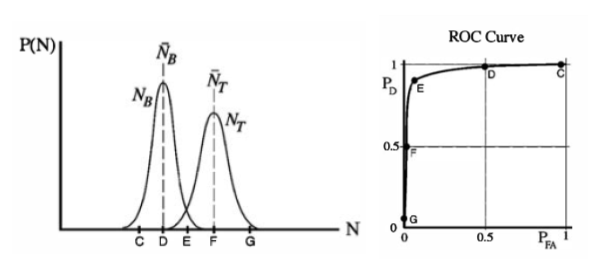
\includegraphics[width=0.7\textwidth]{images/ROC_curve_Knoll.png}
        \caption{The left plot shows the probability of observing a specific count $N$ for background $N_B$ and total count $N_T$ when a true source is present. The right plot is the corresponding ROC curve, where the points C through G designate the results when different choices are made for the decision threshold.}
        \label{fig:ROC_curve_Knoll}
    \end{figure}
    \begin{figure}[ht]
        \centering
        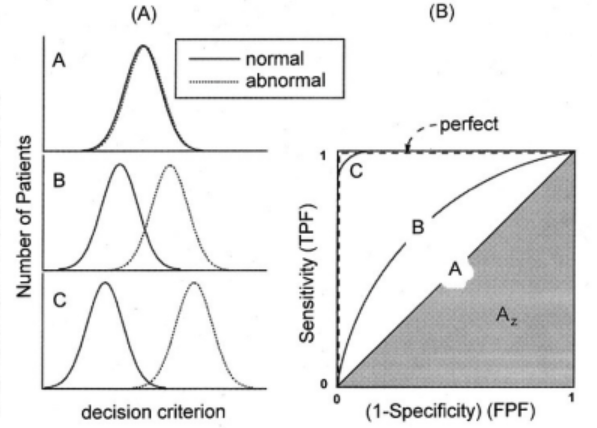
\includegraphics[width=0.5\textwidth]{images/ROC_curve_slides.png}
        \caption{ROC curve with TPF (sensitivity) vs. FPF (1-specificity) }
        \label{fig:ROC_curve_slides}
    \end{figure}
    \item Minimum detectable activity (MDA) - Currie limit\\
    The minimum detectable activity is the smallest net count that can be reported with a certain degree of confidence that it represents a true activity form a sample and not a statistical variation of the background. \\
    Using figure~\ref{fig:ROC_curve_Knoll}, assuming both $N_B$ and $N_T$ are Gaussian, we know:
    \begin{itemize}
        \item[] $N_S=N_T-N_B$
        \item[] $\sigma_{N_S}^2=\sigma^2_{N_T}+\sigma^2_{N_B}$
    \end{itemize}
    \begin{figure}[ht]
        \centering
        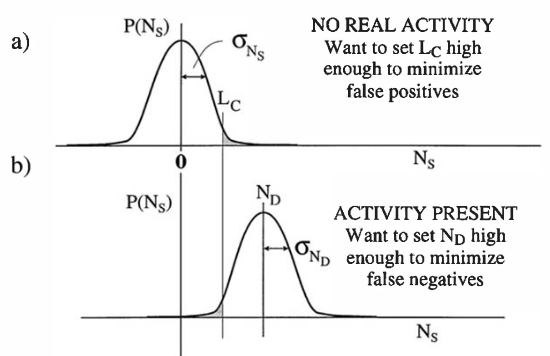
\includegraphics[width=0.5\textwidth]{images/currie_limit.png}
        \caption{Currie limit calculation.}
        \label{fig:currie_limit}
    \end{figure}
    \begin{enumerate}
        \item No real activity is present:
        \begin{itemize}
            \item If there is no real activity in the sample, then the true mean value of $N_S$ is $0$ (shown in figure~\ref{fig:currie_limit}(a), and the true means of $N_B$ and $N_T$ are equal.
            \item Also, $\sigma_{N_T}=\sigma_{N_B}$, and $\sigma_{N_S}=\sqrt{2\sigma^2_{N_B}}=\sqrt{2}\sigma_{N_B}$\\
            If fluctuations are only from counting statistics, $\sigma_{N_S}=\sqrt{2}\sigma_{N_B}=\sqrt{2}\sqrt{N_B}$
            \item Since there is no true activity, any positive indication will be a false positive. We know that in a Gaussian distribution, a random value will fall between the mean $\pm1.64\sigma$ with 90\% probability. Since we are concerned only with positive deviations from the mean (any negative measured $N_S$ value is interpreted as no true activity present), we would have 95\% confidence that a sample is not contaminated if $N_S<L_C=1.64\sigma_{N_S}=1.64\sqrt{2}\sqrt{N_B}=2.33\sqrt{N_B}$ 
            \item For example, with $N_B=100$, then $L_C=23$,\\
            if the measurement yields less than 124 counts, we can assume that it is just background with 95\% confidence.
        \end{itemize}
        \item Real activity is present:
        \begin{itemize}
            \item If we now presume that $N_S>0$ (figure~\ref{fig:currie_limit}(b)), any conclusion that there is no true activity present would be a false negative. 
            \item How large does $N_S$ have to be to make false negatives unlikely? If $N_S=L_C$, the probability of a false negative would be 50\%.
            \item In the Currie definition, a 5\% false-negative probability is chosen. Let $N_D$ be the minimum value of $N_S$ that meets this criterion.\\
            $N_D=L_C+1.64\sigma_{N_D}$
            \item $\sigma^2_{N_D}=\sigma^2_{N_T}+\sigma^2_{N_B}=N_T+N_B=N_D+2N_B$\\
            $\sigma_{N_B}=\sqrt{N_D+2N_B}$\\
            With $L_C=1.64\sqrt{2}\sqrt{N_B}$ , $N_D=1.64(\sqrt{2N_B}+\sqrt{N_D+2N_B})$\\
            $\Rightarrow\;N_D=4.65\sqrt{N_B}+2.71$
            \item For example, with $N_B=100$, then $N_D=49$,\\
            if the measurement yields more than 149 counts, we have 95\% confidence that it is a true signal. 
        \end{itemize}
    \end{enumerate}
\end{enumerate}